% \usepackage{tikz}
% \usetikzlibrary{arrows,shapes.gates.logic.US,shapes.gates.logic.IEC,calc}
\hbadness=100000000
\hfuzz=150pt
\documentclass{article}
% \usepackage{circuitikz}
\title{Homework 3}
\author{
	Nathaniel Thomas\\
	\texttt{A17069898}
}
\usepackage{amsmath}
\usepackage[table,x11names]{xcolor}
\usepackage{circuitikz}
\usetikzlibrary{calc}

\newcommand*\xor{\oplus}
\begin{document}
\maketitle

\begin{enumerate}
	\item \begin{enumerate}
		      \item
		            \begin{align*}
			             & (x_3 \land x_2 \land \lnot x_1 \land \lnot x_0) \lor
			            (\lnot x_3 \land x_2 \land x_1 \land \lnot x_0) \lor
			            (\lnot x_3 \land \lnot x_2 \land \lnot x_1 \land \lnot x_0) \\
			             & = \lnot x_0 \land \left[
				            (x_3 \land x_2 \land \lnot x_1  ) \lor
				            (\lnot x_3 \land x_2 \land x_1  ) \lor
				            (\lnot x_3 \land \lnot x_2 \land \lnot x_1 )
			            \right]                                                     \\
			             & = \lnot x_0 \land \left[
				            x_2 \land ( (x_3 \land \lnot x_1) \lor (\lnot x_3 \land x_1) ) \lor
				            (\lnot x_2 \land \lnot x_3 \land \lnot x_1 )
			            \right]                                                     \\
			             & = \lnot x_0 \land \left[
				            x_2 \land (x_3 \xor x_1) \lor
				            \lnot (x_2 \lor  x_3 \lor x_1 )
			            \right]                                                     \\
			            % & =
			            %  & = \lnot x_0 \land \left[
			            %  x_2 \land (x_3 \xor x_1) \lor \lnot x_2 \land (\lnot x_3 \land  \lnot x_1)
			            % \right]                                                     \\
			            %  & =\lnot x_0 \land \left[
			            %  x_2 \land (x_3 \xor x_1) \lor \lnot x_2 \land \lnot (x_3 \lor  x_1)
			            % \right]                                                     \\
			            %  & =\lnot x_0 \land \left[
			            %  x_2 \land (x_3 \xor x_1) \lor \lnot (x_2 \lor x_3 \lor  x_1)
			            % \right]                                                     \\
		            \end{align*}

		      \item ~

		            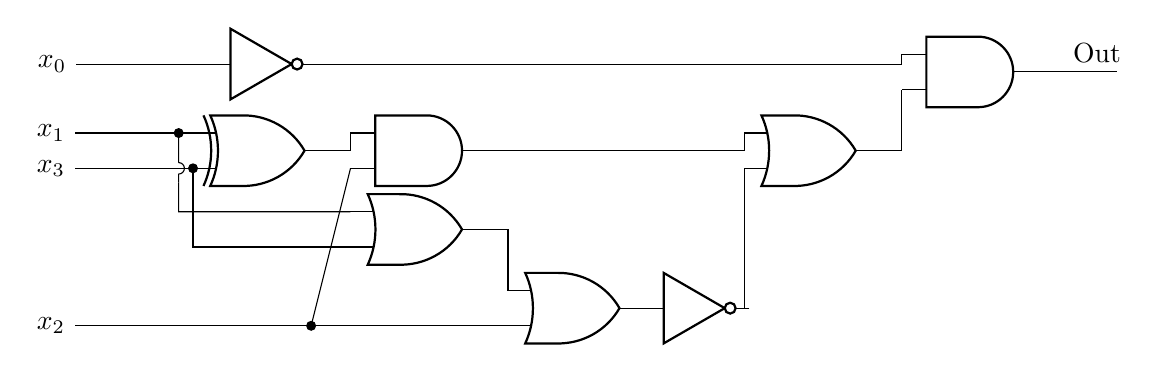
\begin{tikzpicture}
			            \ctikzset{
				            logic ports=ieee,
				            logic ports/scale=0.8,
				            % logic ports/fill=black
			            }

			            \node[not port] (not1) at (0,-0.9){};
			            \node[xor port] (xor1) at (0, -2){};
			            \node[or port] (or1) at (4, -4){};
			            \node[or port] (or2) at (2, -3){};
			            \node[and port] (and1) at (2, -2){};
			            \node[not port] (not2) at (5.5, -4){};
			            \node[or port] (or3) at (7, -2){};
			            \node[and port] (and3) at (9, -1){};

			            \draw (not1.in) --   ++ (-1.65,0)node[left](x0){$x_0$};
			            \draw (xor1.in 1) -- ++ (-1.5,0)node[left](x1){$x_1$};
			            \draw (xor1.in 2) -- ++ (-1.5,0)node[left](x3){$x_3$};
			            \draw (or1.in 2) --  ++ (-5.5,0)node[left](x2){$x_2$};
			            % \draw (and1.in 2) -| ++(-0.5,-2)(x2);
			            \draw (xor1.out) -| (and1.in 1);
			            \draw (or2.out) -| (or1.in 1);
			            \draw (or1.out) -- (not2.in);
			            \draw (not2.out) -| (or3.in 2);
			            \draw (and1.out) -| (or3.in 1);
			            \draw (not1.out) -| (and3.in 1);
			            \draw (or3.out) -| (and3.in 2);
			            \draw (and1.in 2) to[short,-*] ++(-0.5,-2)(x2);
			            \draw (and3.out) -- ++(1,0) node[near end,above]{Out};

			            \node at (xor1.in 2)
			            [
				            below,
				            jump crossing,
				            rotate=-90,
				            scale=1.3
			            ](X){};

			            \draw (or2.in 1) -| (X.east)
			            (X.west) to[short,-*] (X.west |- xor1.in 1);

			            \node at (xor1.in 2)[anchor=east](Y){};
			            \draw (or2.in 2) -| (Y.east);
			            \draw (Y.east) to[short,-*] (xor1.in 2);

			            \node at (or1.in 2)[anchor=east](Z){};
		            \end{tikzpicture}



		      \item \begin{enumerate}
			            \item No, because $P_1((1, 0, 1, 0))$ = 1 but the table says that it
			                  is 0.
			            \item The multiples of 6 that are less than 15 (the
			                  maximum value of a 4 digit binary number) are \{0, 6, 12\}.
			                  \begin{align*}
				                  P_2((0,0,0,0)) = 1 \\
				                  P_2((0,1,1,0)) = 1 \\
				                  P_2((1,1,0,0)) = 1 \\
			                  \end{align*}
			                  Because there are only 3 inputs where \textit{out} is 1,
			                  the condition is satisfied and the definition is correct.
			            \item No. Counterexample:
			                  $$
				                  \left[1100\right]_{s,4} = (-4)_{10} \ne (1100)_{2,4} = (12)_{10}
			                  $$
			                  yet \textit{out} for 1100 is 1 (T).
		            \end{enumerate}
	      \end{enumerate}

	\item \begin{enumerate}
		      \item ~


		            \begin{tabular}{|c|c||c|c|c|c|c|c|c|}
			            \hline
			            $x_1$ & $x_0$ & $a$ & $b$ & $c$ & $d$ & $e$ & $f$ & $g$ \\
			            \hline
			                  &       &     &     &     &     &     &     &     \\
			            0     & 0     & 1   & 1   & 1   & 0   & 1   & 1   & 1   \\
			                  &       &     &     &     &     &     &     &     \\
			            \hline
			                  &       &     &     &     &     &     &     &     \\
			            0     & 1     & 1   & 0   & 0   & 1   & 1   & 1   & 0   \\
			                  &       &     &     &     &     &     &     &     \\
			            \hline
			                  &       &     &     &     &     &     &     &     \\
			            1     & 0     & 1   & 0   & 1   & 1   & 1   & 1   & 0   \\
			                  &       &     &     &     &     &     &     &     \\
			            \hline
			                  &       &     &     &     &     &     &     &     \\
			            1     & 1     & 0   & 1   & 1   & 1   & 1   & 1   & 0   \\
			                  &       &     &     &     &     &     &     &     \\
			            \hline
		            \end{tabular}

		      \item From the truth table, we can see that the following hold:
		            \begin{align*}
			            a & = \lnot (x_0 \land x_1)         \\
			            b & = \lnot (x_0 \xor x_1)          \\
			            c & = \lnot (x_0 \xor x_1) \lor x_1 \\
			            d & = x_0 \lor x_1                  \\
			            e & = 1                             \\
			            f & = 1                             \\
			            g & = \lnot (x_0 \lor x_1)
		            \end{align*}


		            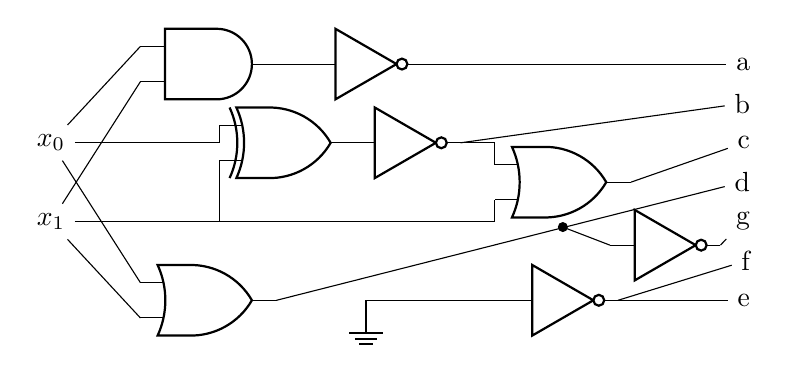
\begin{tikzpicture}
			            \ctikzset{
				            logic ports=ieee,
				            logic ports/scale=0.8,
				            % logic ports/fill=black
			            }
			            \node[and port] (and1) at (2,0){};
			            \node[not port] (not1) at (4, 0){};
			            \draw (and1.out) -- (not1.in);

			            \node[xor port] (xor1) at (3,-1){};
			            \node[not port] (not2) at (4.5, -1){};
			            \draw (xor1.out) -- (not2.in);

			            % \node[not port] (not3) at (4, -2){};
			            \node[or port] (or1) at (2, -3){};

			            \node (x0) at (0,-1){$x_0$};
			            \node (x1) at (0,-2){$x_1$};

			            \draw (x0) -| (xor1.in 1);
			            \draw (x1) -| (xor1.in 2);
			            % \draw (x1) -- (not3.in);

			            \draw (x0) -- (and1.in 1);
			            \draw (x1) -- (and1.in 2);

			            \draw (x0) to[short] (or1.in 1);
			            \draw (x1) to[short] (or1.in 2);

			            \node[or port] (or2) at (6.5, -1.5){};
			            \draw (not2.out) -| (or2.in 1);
			            \draw (x1) -| (or2.in 2);
			            % \draw (not3.out) -| (and2.in 2);

			            \node[left] (a) at (9,0) {a};
			            \node[left] (b) at (9,-0.5){b};
			            \node[left] (c) at (9,-1){c};
			            \node[left] (d) at (9,-1.5){d};
			            \node[left] (g) at (9,-2){g};
			            \node[left] (f) at (9,-2.5){f};
			            \node[left] (e) at (9,-3){e};



			            \draw (not1.out) -- (a);
			            \draw (not2.out) -- (b);
			            \draw (or2.out) -- (c);
			            \draw (or1.out) -- (d);
			            \node[not port] (not4) at (6.5,-3){};
			            \node[ground] (gr) at (4,-3){};
			            \draw (gr) -- (not4.in);
			            \draw (not4.out) -- (e);
			            \draw (not4.out) -- (f);
			            \node[not port] (not5) at (7.8, -2.3){};
			            % \draw (g) to[short,-*] (6.5,-2.07);
			            \draw (not5.in) to[short,-*] (6.5,-2.07);
			            % \draw (6.5,-2.07) to[short,-*] (not5.in);
			            \draw (not5.out) -- (g);
		            \end{tikzpicture}

	      \end{enumerate}

	\item \begin{enumerate}
		      \item ~


		            \begin{tabular}{|c|c|c||c|}
			            \hline
			            p & q & r &   \\
			            \hline
			            1 & 1 & 1 & 0 \\
			            \hline
			            1 & 1 & 0 & 1 \\
			            \hline
			            1 & 0 & 1 & 1 \\
			            \hline
			            1 & 0 & 0 & 0 \\
			            \hline
			            0 & 1 & 1 & 0 \\
			            \hline
			            0 & 1 & 0 & 0 \\
			            \hline
			            0 & 0 & 1 & 0 \\
			            \hline
			            0 & 0 & 0 & 0 \\
			            \hline
		            \end{tabular}

		      \item ~

		            \begin{tabular}{|c|c|c||c|}
			            \hline
			            p & q & r &   \\
			            \hline
			            1 & 1 & 1 & 1 \\
			            \hline
			            1 & 1 & 0 & 1 \\
			            \hline
			            1 & 0 & 1 & 1 \\
			            \hline
			            1 & 0 & 0 & 0 \\
			            \hline
			            0 & 1 & 1 & 1 \\
			            \hline
			            0 & 1 & 0 & 1 \\
			            \hline
			            0 & 0 & 1 & 1 \\
			            \hline
			            0 & 0 & 0 & 0 \\
			            \hline
		            \end{tabular}

		      \item ~


		            \begin{tabular}{|c|c|c||c|}
			            \hline
			            p & q & r &   \\
			            \hline
			            1 & 1 & 1 & 1 \\
			            \hline
			            1 & 1 & 0 & 1 \\
			            \hline
			            1 & 0 & 1 & 1 \\
			            \hline
			            1 & 0 & 0 & 1 \\
			            \hline
			            0 & 1 & 1 & 1 \\
			            \hline
			            0 & 1 & 0 & 1 \\
			            \hline
			            0 & 0 & 1 & 0 \\
			            \hline
			            0 & 0 & 0 & 1 \\
			            \hline
		            \end{tabular}
	      \end{enumerate}
	\item \begin{enumerate}
		      \item Let \textit{c, d, p} and $f$ represent the guilt of the cat, dog,
		            pig, and frog, respectively. Then
		            \begin{align}
			             & \lnot c \to d             \\
			             & \lnot c \leftrightarrow f \\
			             & \lnot d \to p             \\
			             & \lnot c \to p             \\
		            \end{align}
		            This implies the following
		            \begin{align}
			             & \lnot c \to d \land p
		            \end{align}
		            Because all of the other characters are now linked to the
		            cat, we can analyze two cases: one where the cat is
		            guilty, and another where it is innocent. If innocent,
		            we know from (6) and (2) that the dog and pig are
		            guilty, and the frog is innocent. If the cat is
		            guilty, we only \textit{know} that the frog is guilty from (2).
		            However, there is no restriction on $p$ or $d$. So
		            they can be (T,T), (T,F), or (F,T).

		            We can arrive at the same conclusion using a truth
		            table with the previous equations written in terms of
		            $\land, \lor, \xor, $ and $\lnot$, which shows 4
		            consistent scenarios.

		            \begin{tabular}{|c|c|c|c||c|c|c|c|}
			            \hline
			            c                   & d & p & f & $c \lor d$ & $\lnot(c\xor f)$ & $d \lor p$ & $c \lor p$ \\
			            \hline
			            \rowcolor{yellow} T & T & T & T & T          & T                & T          & T          \\
			            T                   & T & T & F & T          & F                & T          & T          \\
			            \rowcolor{yellow} T & T & F & T & T          & T                & T          & T          \\
			            T                   & T & F & F & T          & F                & T          & T          \\
			            \rowcolor{yellow}T  & F & T & T & T          & T                & T          & T          \\
			            T                   & F & T & F & T          & F                & T          & T          \\
			            T                   & F & F & T & T          & T                & F          & T          \\
			            T                   & F & F & F & T          & F                & F          & T          \\
			            F                   & T & T & T & T          & F                & T          & T          \\
			            \rowcolor{yellow}F  & T & T & F & T          & T                & T          & T          \\
			            F                   & T & F & T & T          & F                & T          & F          \\
			            F                   & T & F & F & T          & T                & T          & F          \\
			            F                   & F & T & T & F          & F                & T          & T          \\
			            F                   & F & T & F & F          & T                & T          & T          \\
			            F                   & F & F & T & F          & F                & F          & F          \\
			            F                   & F & F & F & F          & T                & F          & F          \\
			            \hline
		            \end{tabular}

		            Therefore, we do not have enough information to conclude who was involved in the crime.

		      \item The guilt of the pig only helps us rule out 1 out of the 4 scenarios. This is because
		            we can only draw conclusions from the \textit{innocence} of the pig, which using the
		            following equations
		            \begin{align*}
			            \lnot p \to d \\
			            \lnot p \to c \\
			            c \leftrightarrow f
		            \end{align*}
		            would help us conclude that the cat, dog, and frog are guilty.

		            Using the truth table, we see that out of the 4 consistent possibilities,
		            only one is ruled out with the guilt of the pig, leaving all of the following
		            open:

		            \begin{tabular}{|c|c|c|c||c|c|c|c|}
			            \hline
			            c & d & p & f & $c \lor d$ & $\lnot(c\xor f)$ & $d \lor p$ & $c \lor p$ \\
			            \hline
			            T & T & T & T & T          & T                & T          & T          \\
			            T & F & T & T & T          & T                & T          & T          \\
			            F & T & T & F & T          & T                & T          & T          \\
			            \hline
		            \end{tabular}

		            This means we still do not have enough information to conclude who was
		            involved in the crime.
	      \end{enumerate}
\end{enumerate}



\end{document}
